
\section{Graphical User Interface}

\subsection{Introduction}
My goal was to make an easy to use interface, where the possible users of these devices can access their network and can manage their devices efficiently. On the other hand this solution gives an informative, nice looking visualisation page. Because Thread Network can be connected to the internet, I chose a Webpage as a GUI to use.

\subsection{Programs used for the website}
The interface is implemented with a webpage, which I create with \textit{Bootstrap CSS}, \textit{HTML} and on the client side I use \textit{JavaScript} to check the integrity of the data. On the server side, I use \textit{FastAPI} as backend, which is one of the fastest Python frameworks currently available. Thanks to the Python language
\begin{itemize}
    \item it can be developed quickly, 
    \item because of the python's syntactics is less chance of bugs from typos,
    \item it is easy to learn,
    \item it can be developed in relatively short code, avoiding unnecessary code duplication.
\end{itemize}
\clearpage
\noindent
Furthermore, FastAPI is characterized by
\begin{itemize}
    \item it is robust, produces automatic documentation and is easy to debug,
    \item it is based on JSON schema and OpenAPI.
\end{itemize}
I run the website on a \textit{Asynchronous Server Gateway Interface} (short \textbf{ASGI}) web server which called \textit{Uvicorn}. Essentially, this creates the connection between the backend and the web server. That is, in the event that an HTTP request is received from the client, the web server will signal this to FastAPI. All communication between the program and the server will be done in a Python Dictionary format, which is a data structure. A Dictionary is similar to the JSON data format, which is stored as text, whereas a Dictionary is a memory object.
I implement the dynamically changing web page elements with \textit{Jinja template}. This program does the processing of the data from the Dictionary objects and pastes it into the appropriate location into the html page. This template language also contains conditional branching and foreach cycles.


\subsection{Database}
Before I get to the backend, I would like to introduce the database model, which I designed.
\begin{figure}[!htb]
    \centering
    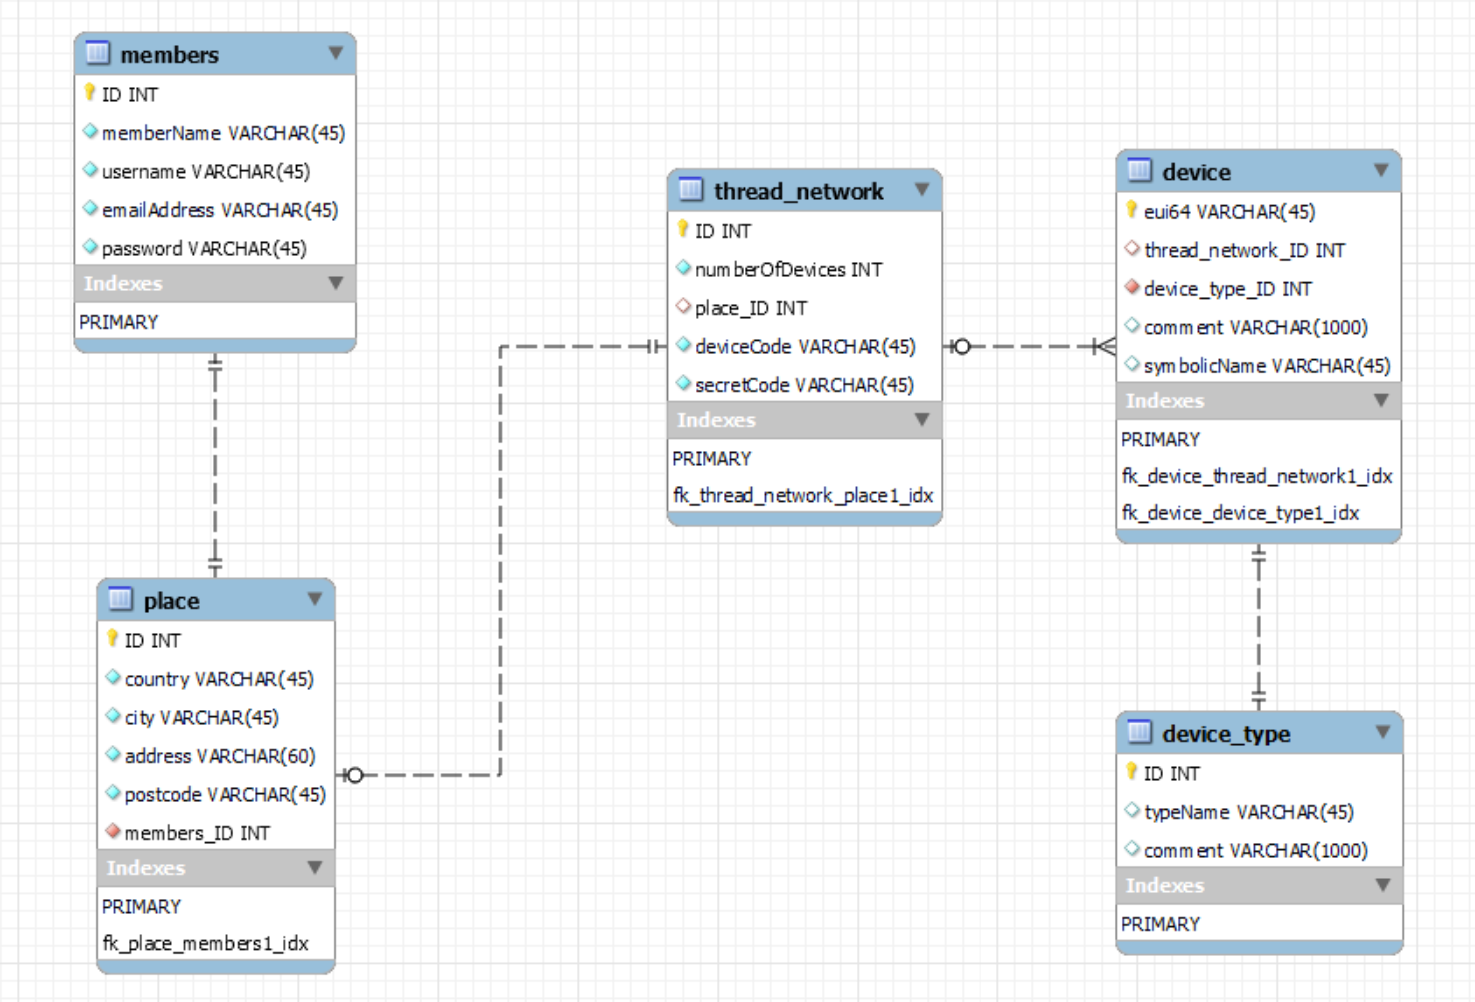
\includegraphics[width=\textwidth]{img/adatbazis.png}
    \caption{The database model}
    \label{fig:database}
\end{figure}

\subsubsection{Users or members}
The data is stored in a \textit{MariaDB} database, which is an Open-Source version of MySQL. Figure \ref{fig:database} shows that there is a separate table for users starting from the top left corner.
For each user, I associate an ID that is automatically incremented and that corresponds to the primary key. A user also has a name, surname combination and an email address, each of which forms a separate column. For faster login, I associate a username with the previous ones and of course a password that the user can enter.

\subsubsection{Place}
I designed my Thread network so, that only one Thread network can exist in one home. I think during this development, more than 16,000 devices are enough for a house. So I store where this apartment is located, geographically in this table. This table already contains an external key, because a house can belong to a user and this connection is implemented by a one-to-one connection.

\subsubsection{Thread network}
Only Border Routers can make Thread networks in this development. All networks should be pre-populated in the database, so that when a user gets access to one, it just have to be registered to the home. Each network has an ID which is also automatically incremented and this is also the primary key. A column contains the number of device connected to a the network, purely for statistical reasons and to deal with the case that someone wants to connect more than 16,000 devices. The registration process is such that each device has a private name, which I call deviceCode in the table and a secret password, which I call secretCode. These can be supplied on a piece of paper with each device.


\subsubsection{Device type}
Each device type has an ID, which is also an automatically incremented primary key and two additional columns. One of these stores the name of the device type, such as the Thread router and optional lamp switch as Blind Access Point described later and the associated comment. In the comment column I store a basic configuration of the device as text. As JSON is easy to handle inside Python, I put the data into a JSON file and convert it to text.
\begin{lstlisting}[language=Python]
    BLIND_ACCESS_POINT_DEVICE_TYPE_STRUCT = {
        "isLampConnected": False,
        "lampstate": False,
        "isExtensionBoardConnected": False,
        "whichExtendedActive": "00000"
    }
\end{lstlisting}

\subsubsection{Devices}
Each device has a unique identifier, similar to the MAC address from the Internet world, only unlike that it is a 64-bit number. This is the eui64 identifier, which I described in an earlier section. Since it is unique for each device I use it as the primary key. Since the devices are also provided by the manufacturer and they do not know which Thread network they will be connected to, the second column in this table will be initialized with NULL, so it is allowed to have the external key take NULL value. This is indicated by the empty red circle. Also the device must have a type and the comment field must be copied to the device with the default settings. This is necessary because if it is a lamp switch then each lamp must have a unique state. This table has a one-to-many relationship with the Thread Network table, since multiple devices can be connected to a network.


\subsection{Backend and website design}
\begin{figure}[!htb]
    \centering
    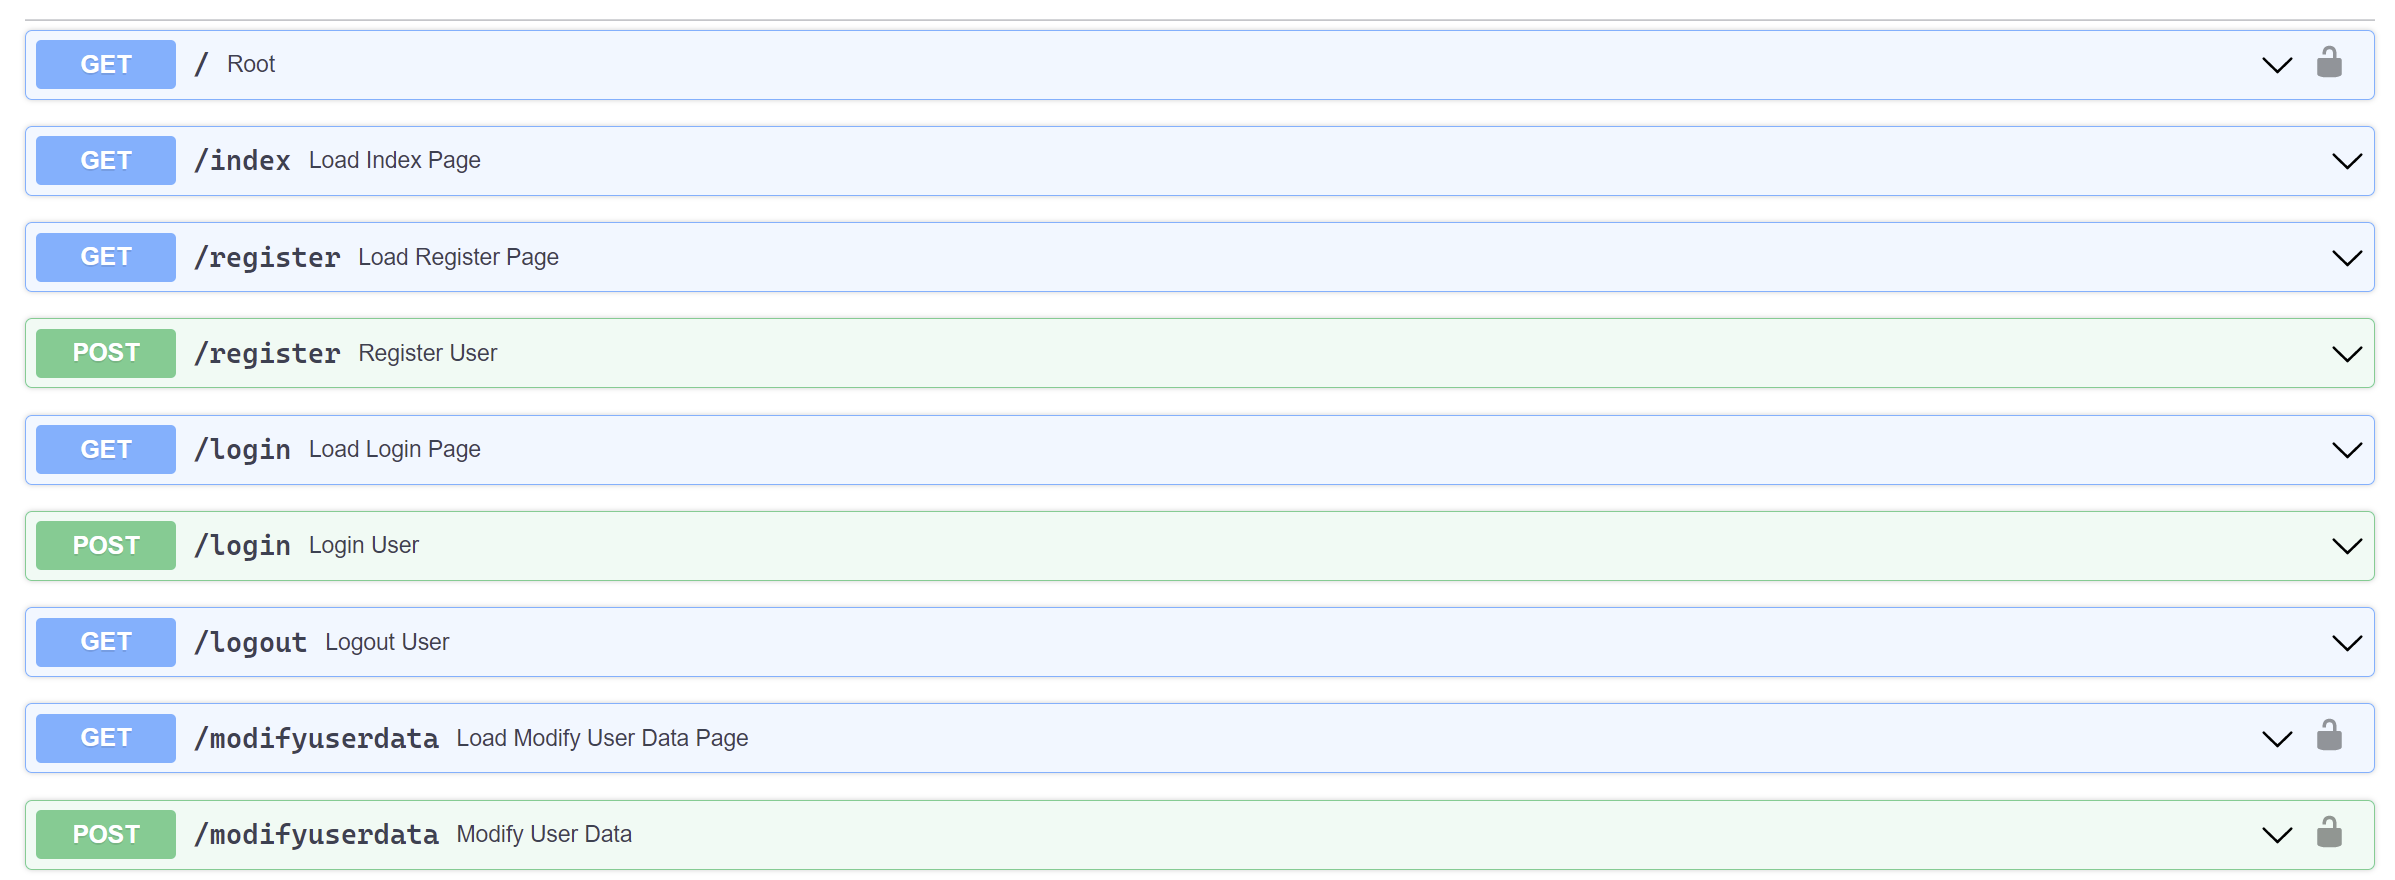
\includegraphics[width=\textwidth]{img/backend.png}
    \caption{Automatic documentation of FastAPI}
    \label{fig:backend}
\end{figure}
\noindent
FastAPI, as I write in the initial listing, produces automatic documentation that the developer can access under "/docs". Part of this documentation is shown in Figure \ref{fig:backend}. On the left side, this documentation shows what queries a particular routine is called for. For example, a registration GET request directs the user to a registration page where HTML forms are found. In the case where all fields are filled in and valid information is provided, a POST request is sent to the same address. Three JavaScript function check the data integrity in the frontend, because of the crash protection and only if all fields are filled in and valid, than the backend executes the query. After a POST request, the data is downloaded from the database and the webpage redirects the user to a feedback page where the user gets informed about the result of the registration process, which may be successful or not, because the passwords do not match or a user already exists.\newline
Where there is a padlock on the right, the website can only be accessed after authentication (\textit{login}). I based the login on the industry standard OAuth2. However, the important information is that the authentication can be done within the HTTP protocol header or with a Cookie. I choose the latter solution and so after login I store the username of the logged-in person and the expiration date of the cookie, which is 24 hours in the browser with a secret key using SHA256 encryption. Before decryption or after decryption, a JSON format will be obtained and that is why it is called \textit{JSON Web Token} or \textbf{JWT}.


\subsection{Frontend}

\subsubsection{Services available to the authenticated user}
\begin{figure}[!htb]
    \centering
    \subfigure[Before logging in]{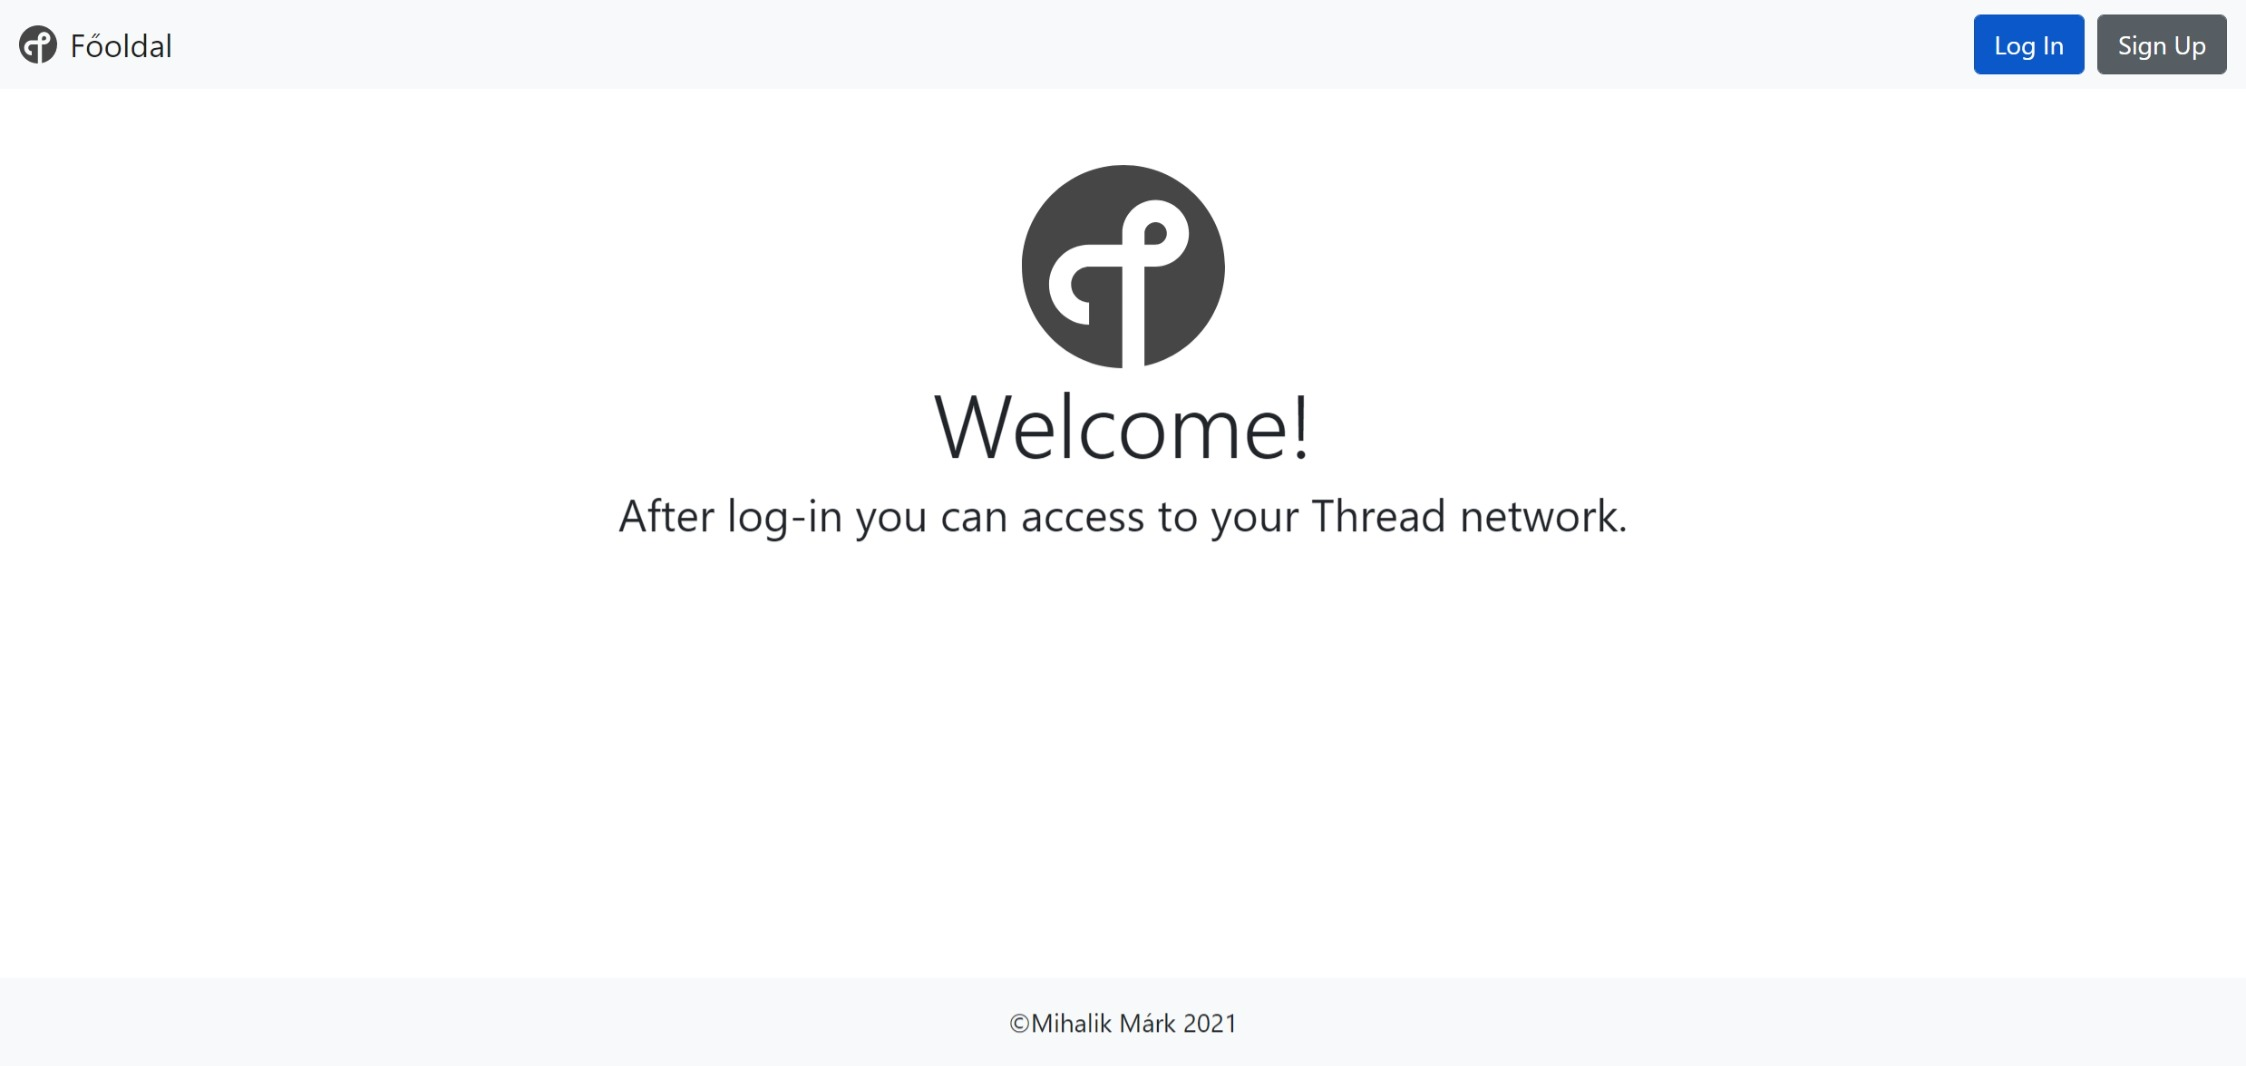
\includegraphics[width=\textwidth]{img/bejelentkezeselott.jpeg}}
    \subfigure[After logging in]{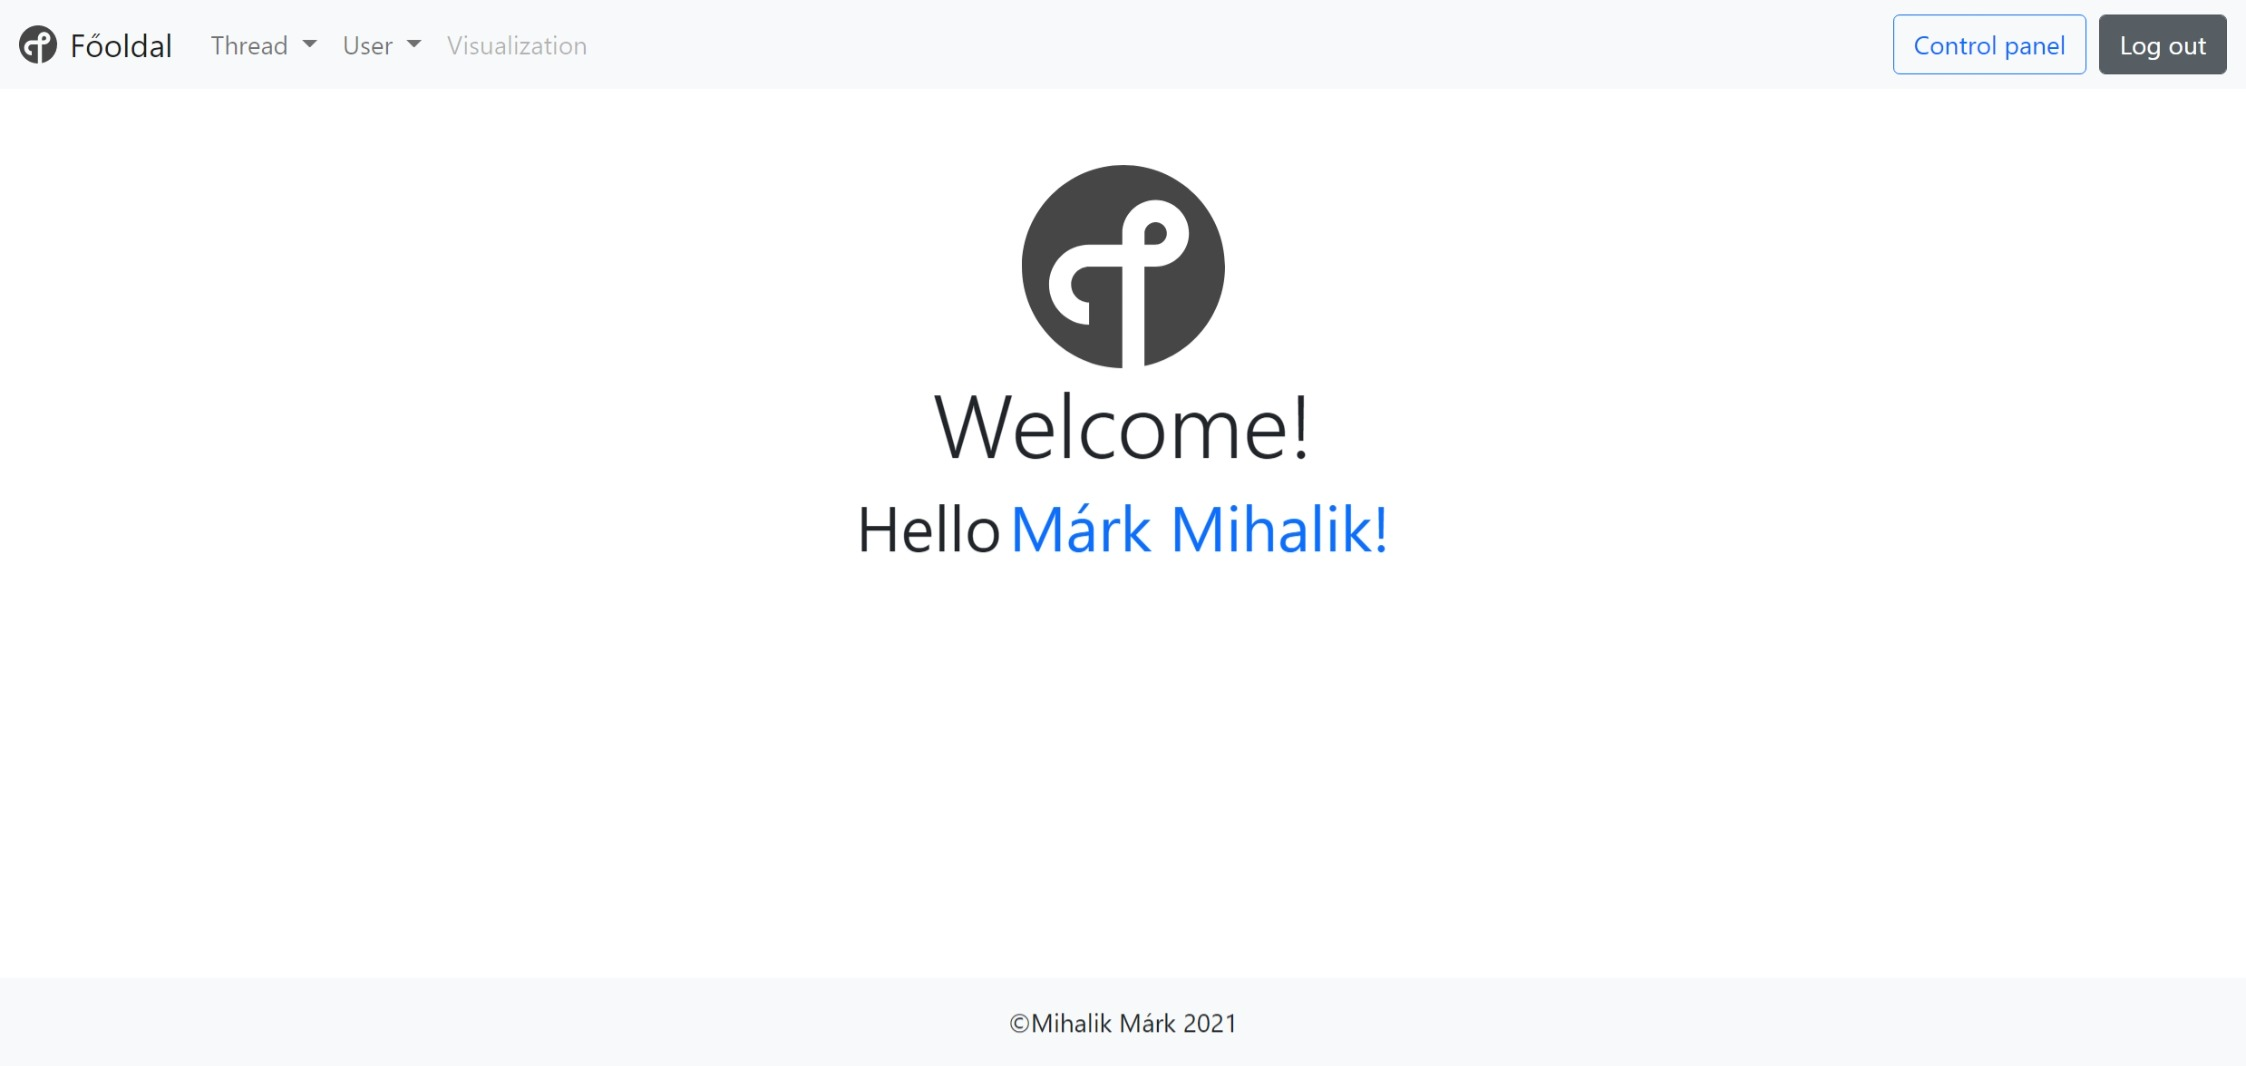
\includegraphics[width=\textwidth]{img/bejelentkezesutan.jpeg}}
    \caption{The main pages of the Webpage}
    \label{fig:welcomepage}
\end{figure}
Figure \ref{fig:welcomepage} shows two pictures of the changes that are available to the user before and after logging in. In the header, there is a change, as dropdown menus appear in the previously empty spaces. The first of these menus is Thread, where the network can be added or possibly deleted. The second dropdown menu is where the user can add location to the personal information or if this information already exists, then the user has the possibility to change it. On the right side, the Login and Register buttons changes after the Log In, as they have been replaced by two other functions, one for the Control Panel and the other for Log Out. 

\subsubsection{Control Panel}
Clicking on this button makes available to the user the devices in the database that belong to the user. As shown in Figure \ref{fig:controlpanel}, there are currently two devices in the database and both devices are Blind Access Points. On one of them the relay that switches the light is active and on the other one it is not, these are indicated by the yellow and white background. The lamps can be removed by software in case, when this device only want to be used as a router or REED.
\begin{figure}
    \centering
    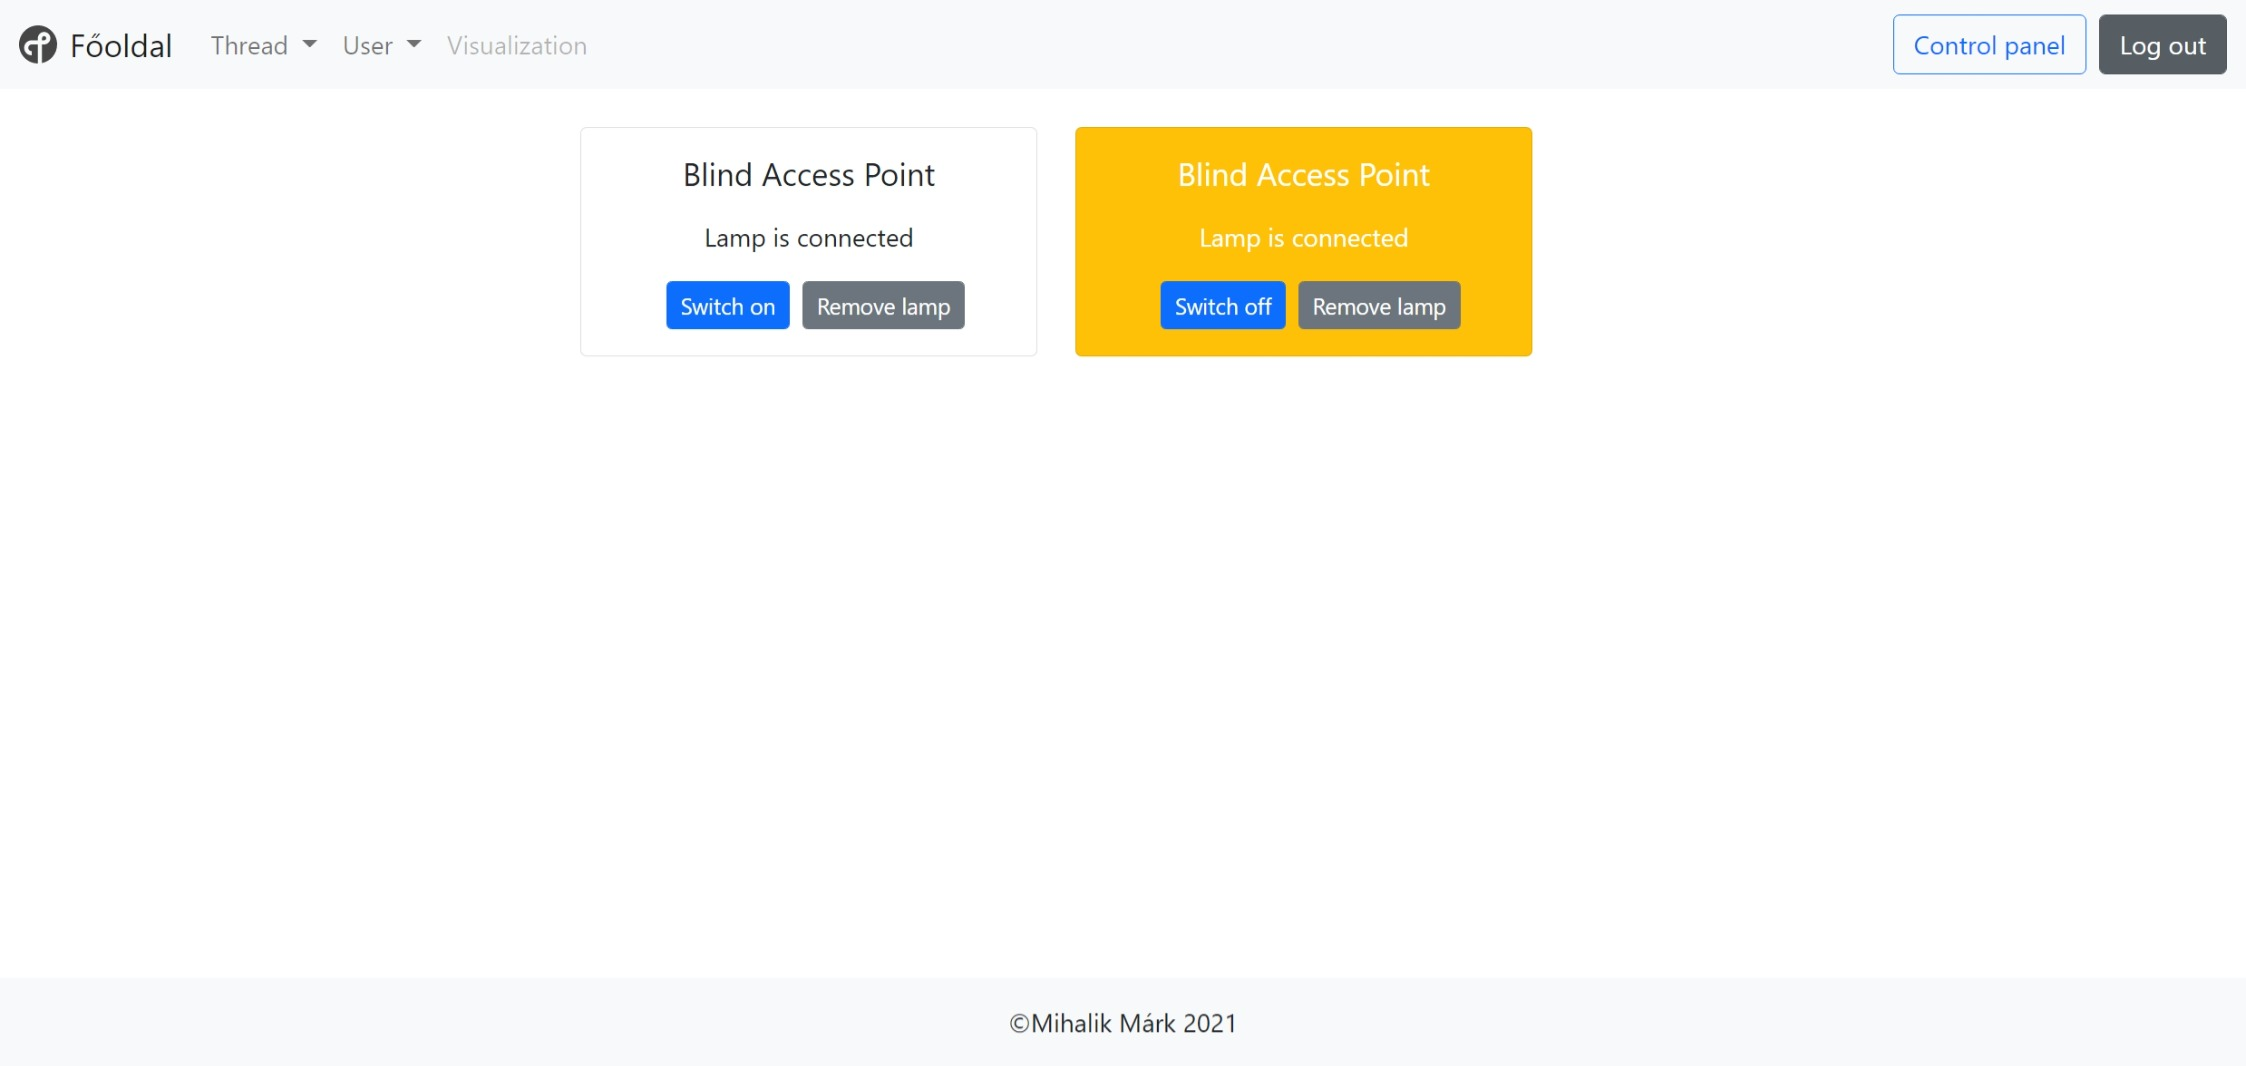
\includegraphics[width=\textwidth]{img/controlpanel.jpeg}
    \caption{The Control Panel}
    \label{fig:controlpanel}
\end{figure}


\subsection{Commissioning}
In this case, to connect a device, a Commissioner is needed on the network. Each connection requires the device's eui64 ID and the device's own password, which is called \textit{Joiner Credential}, which is provided by the programmer in the software created for the device. In my case, this is the Border Router running OpenThread's Commissioner.
Three types of connectivity are thus provided
\begin{itemize}
    \item CLI - Command Line Interface (Linux, MacOS),
    \item Google Commissioner App (Android),
    \item Thread Group Commissioner (Android).
\end{itemize}
The CLI (Command Line Interface) is useful, if the developer wants to test the Thread network and has the eui64 ID and password with a terminal access. Another possible solution is to use the chip's multiprotocol feature, so more protocols can run on the same core, for example a Bluetooth LE and Thread. The second option is a basic Android app by Google that allows QR code connectivity. First, the developer needs an Android smartphone, which is connected to the same home network as the Border Router. Once it appears and the password, that has been created before the network creation is entered. Border Router creates the network itself so according to my Thread network design the manufacturer need to supply this password. The device can join after the QR code reading process is successful. The QR code must contain the eui64 and the joiner password.
\newline
Not much different from this solution is the application published and developed by the Thread Group, which has a much nicer design. Since this is the official app, I use it to connect.
The QR code is generated using the following format:
\begin{center}
    v=1\&\&eui=f4ce36f38f1c9836\&\&cc=BBBBBBBB    
\end{center}
I would like to comment this text, which contains three different part. The first is the version number, since the first version of the Thread is available. The second is eui64 and the third is the password. To generate the code, I use a free Open-Source Program called Zint Barcode Studio\cite{zintdownload}. The QR code must be created according to the ISO18004 standard, where UTF-8 must be chosen as the encoding for the text, or else the app will not be able connect the device.
\begin{figure}[!htb]
    \centering
    
\includegraphics[width=5cm]{img/LampNodeUTF8QRCode5x.png}
    \caption{QR code to connect}
    \label{fig:qrcode}
\end{figure}

\subsection{ThreadGroup application}
\begin{figure}[!htb]
    \centering
    \subfigure[Thread Border Routers]{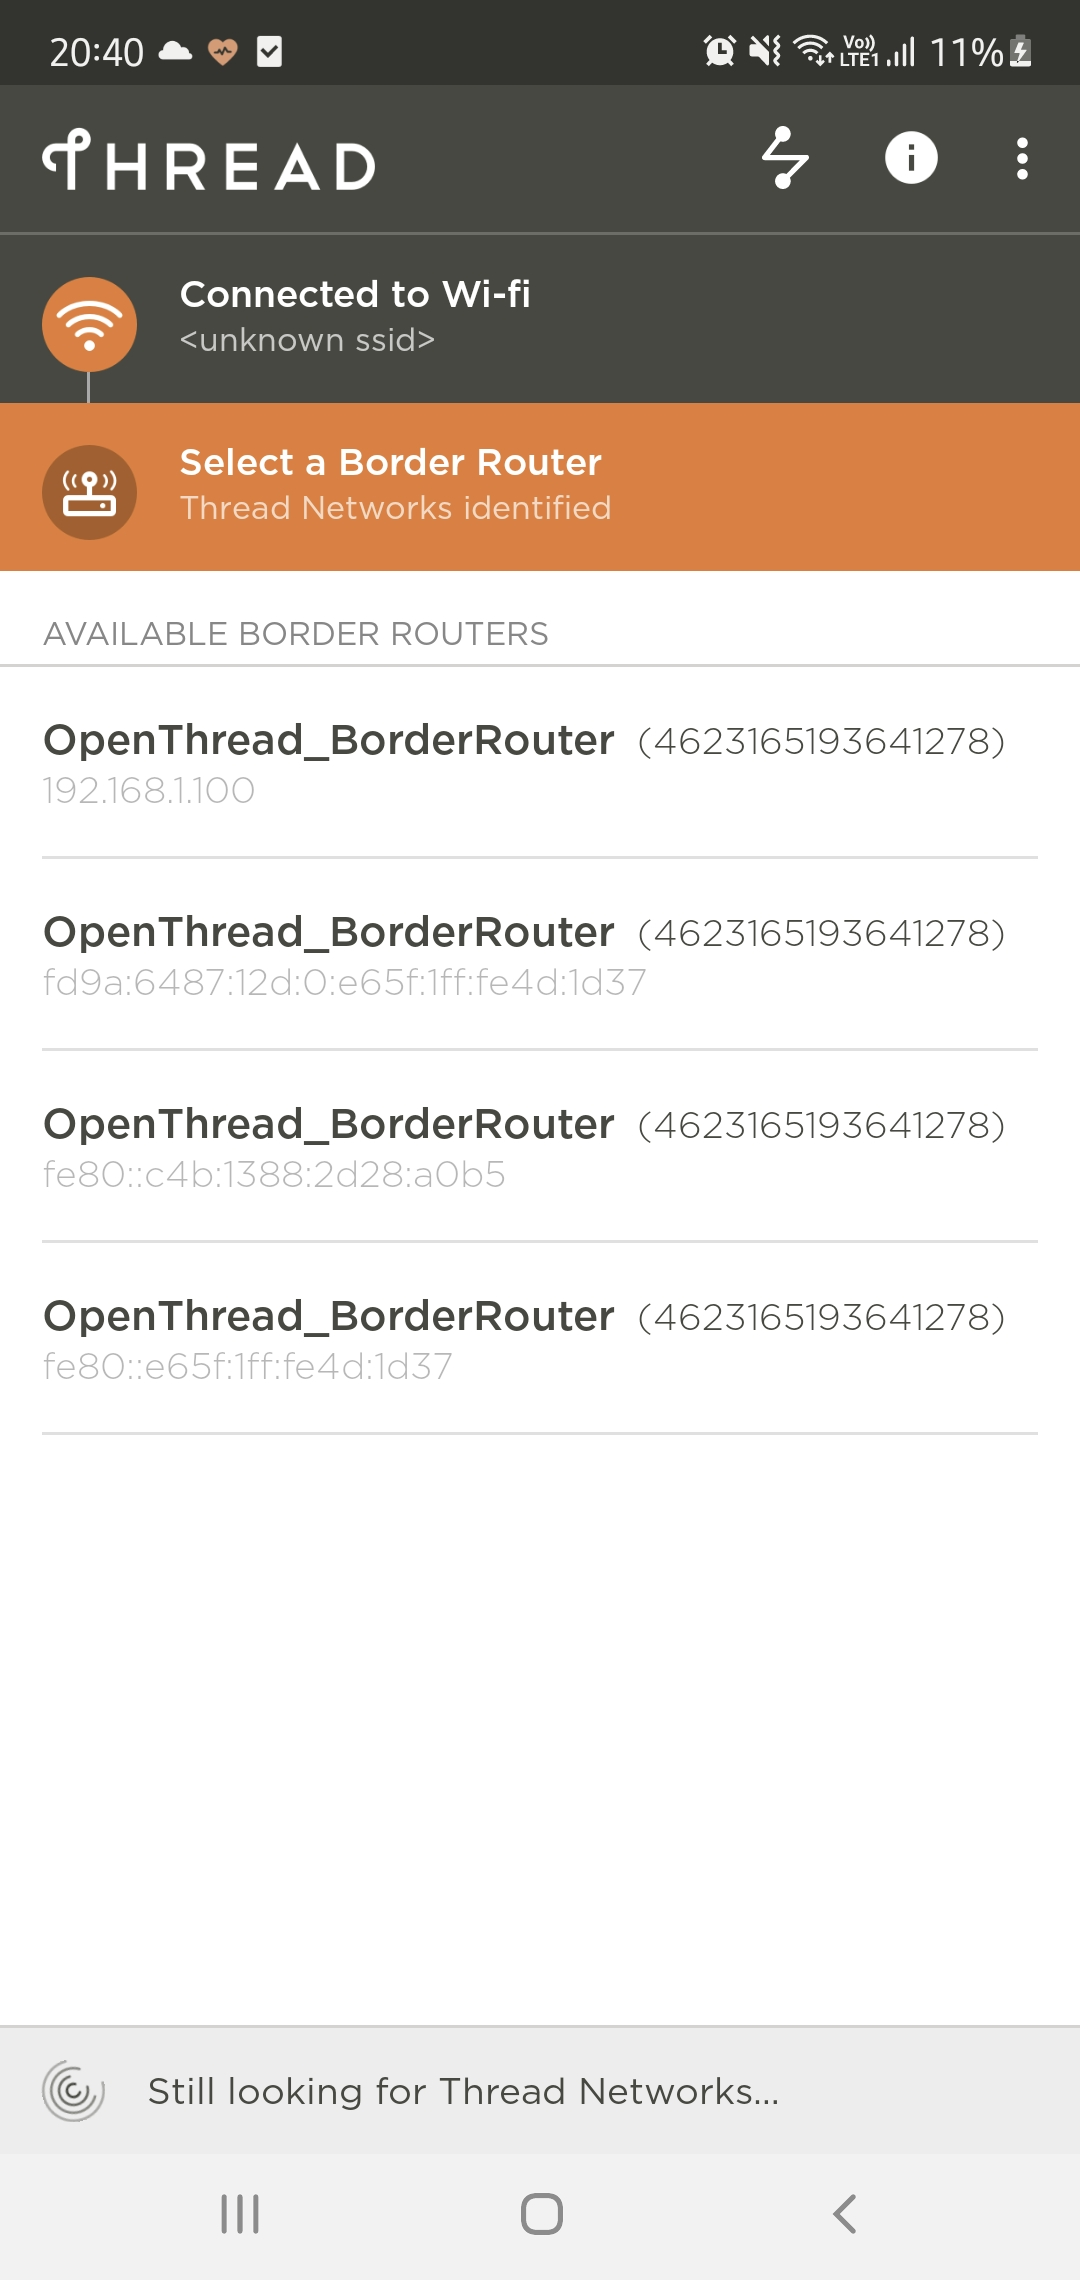
\includegraphics[width=0.3\textwidth]{img/borderouterek.jpg}}
    %\hfill
    \subfigure[Commissioned devices]{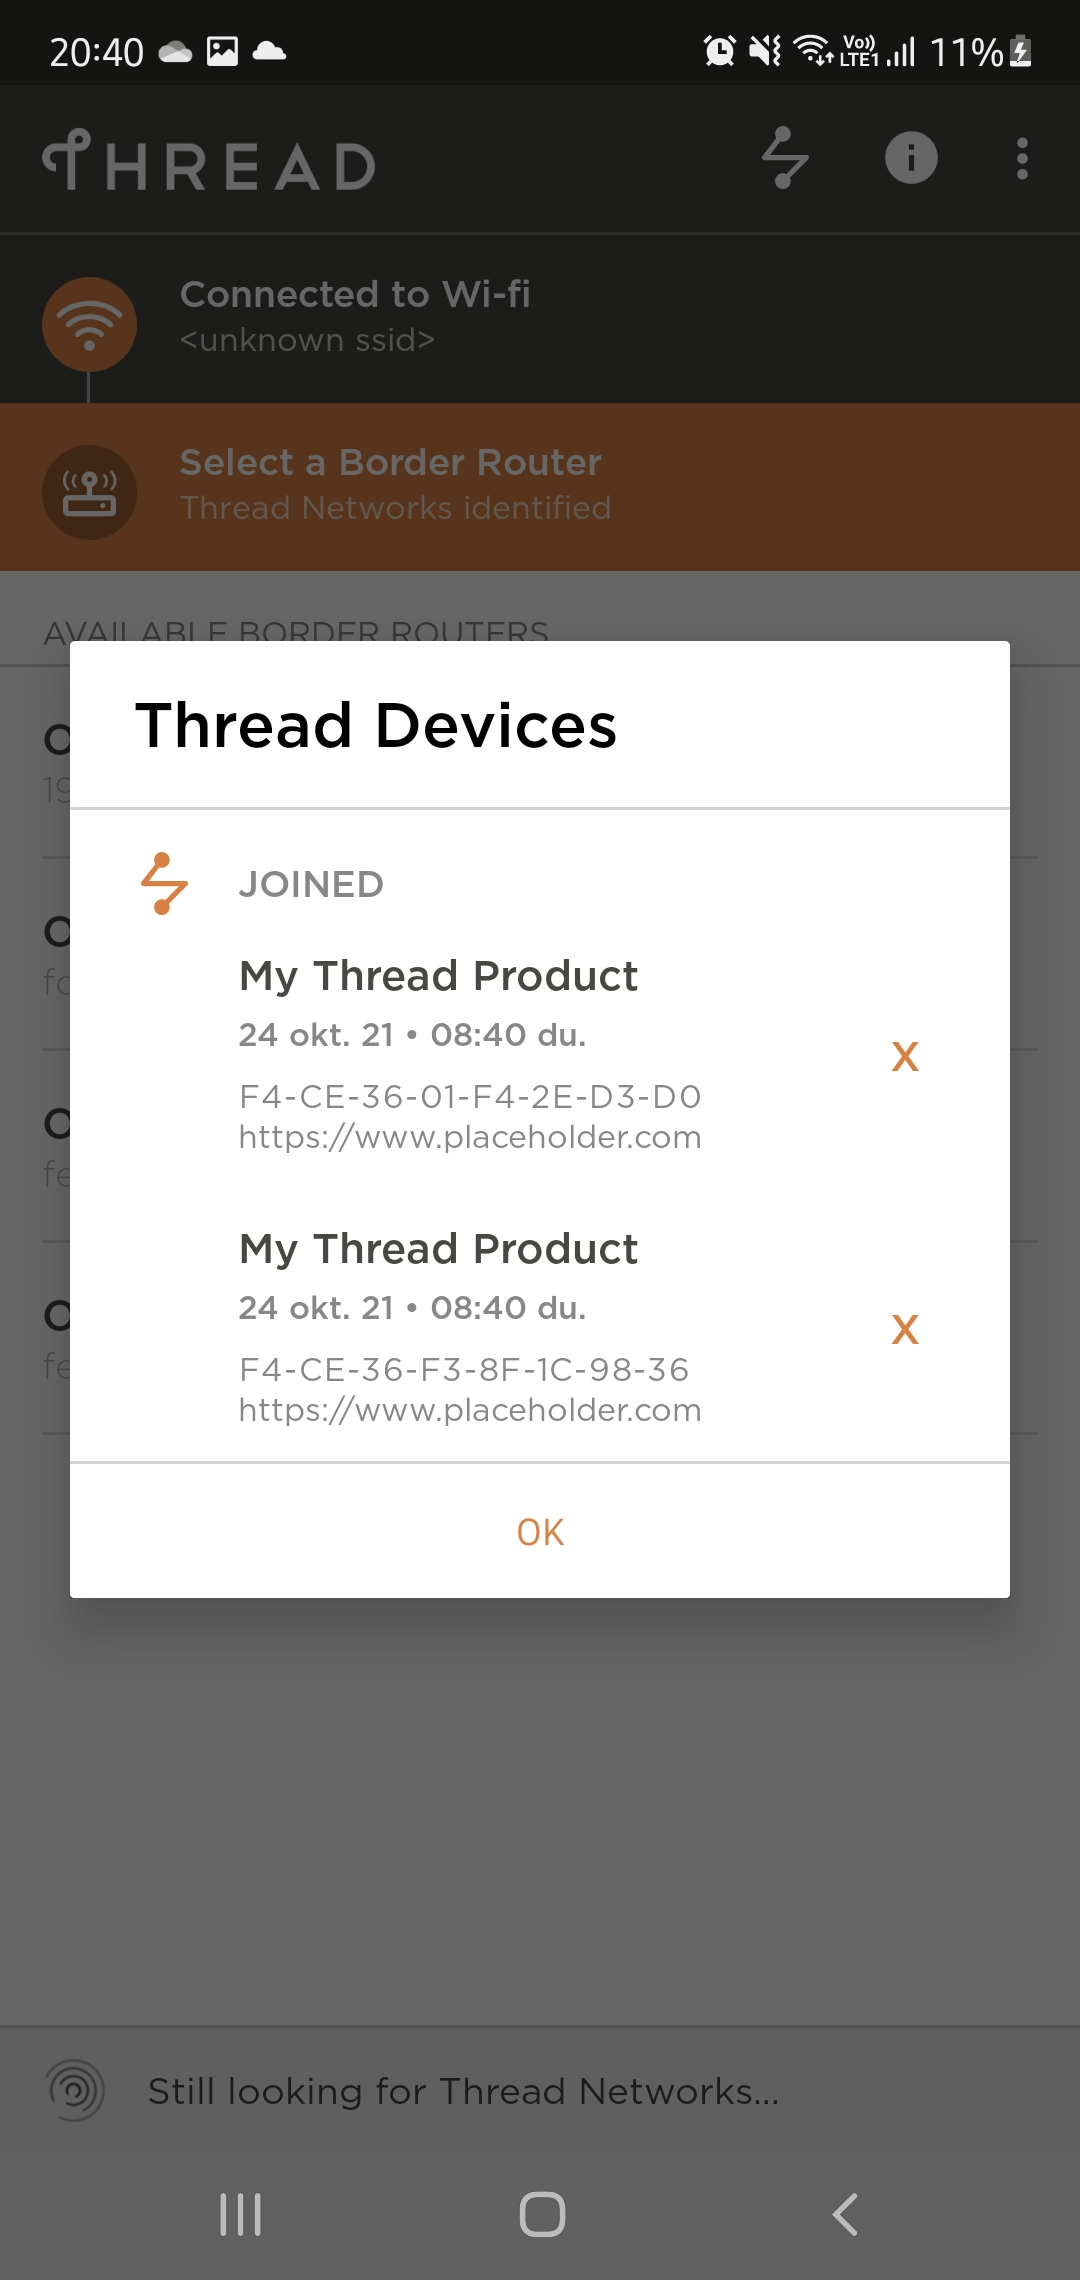
\includegraphics[width=0.3\textwidth]{img/threadeszkozok.jpg}}
    \caption{Thread Group application}
    \label{fig:application}
\end{figure}
Using the app is very simple. As soon as the users are connected to their home network with their Android smartphone, the search for the gateway starts. On the left side of the Figure \ref{fig:application}, can be seen that the one Border Router is available on the home network, which is located at IPv4 address 192.168.1.100. Also, the three other IPv6 addresses below this one belong to the same device. Once one of these is selected, a pop-up window will ask the user to enter the password used to create the Thread network. After the authentication, a QR code scanner will appear on the screen and if the user use it to scan the QR code for the device, which desired to connect, the Commissioner will start. After a few seconds, if the connection is successful, a tick will appear on the display. By clicking on the innermost element of the right navigation bar of the application (a zig-zag line connecting two points) a pop-up window will appear. It is similar to the one shown in the right of Figure \ref{fig:application} with a list of all the devices connected to the Thread network. The user can then remove devices from the network here.

\subsection{Summary of the user interface}
In this section I presented the GUI where the users can be informed the state of their own network and own devices via dynamically changeable cards. I introduced the database model and the Python backend. I also demonstrated a possible solution to the connection process in a Thread network with a smartphone.